\section{Current State}\label{sec:current-state}

This preliminary study design pattern selection was investigated using an AI-assisted tool, ChatGPT, to suggest design patterns using scenarios from existing exam questions. The tool answers are accurate, correct in 93\% of the cases, and always mention specific details of the scenarios, which guide the pattern implementation. In some cases, the answers also included information on classes, interfaces, and methods to be created, which we believe could be improved even more using prompt engineering techniques~\cite{White2023}. Another finding is that wrong answers, even if given in only a few cases, could be misleading and lead the developers in a direction that does not help the design problem described. 

In conclusion, this study suggests that AI-assisted tools can be a valuable resource for developers in understanding and applying design patterns; however, they should not replace human expertise, and the solutions should be reviewed before adoption.

\section{Next Steps}\label{sec:next-steps}

In the next phase of this research project, we will delve into the practical applications of AI-assisted tools, exploring how they address real-world challenges in making software design decisions. This will be done through a multiple case study approach involving at least three companies.

Each company in this study will help us identify and define a complex design problem they are currently facing. These challenges will not only test the abilities of the AI tools we are evaluating. However, they will also provide us with a rich context spanning the many facets and complexities of real-life software design and architecture.

After specifying these issues, we will test three different AI tools. We will send them to each AI tool using prompts that encapsulate the design challenges. This rigorous approach will allow us to assess how each AI model responds to the same problem, thereby exploring the range of solutions that AI can provide.

Responses generated by these AI tools will be meticulously evaluated. We will compare the different tools' responses, aiming to highlight their strengths, weaknesses, and areas of applicability. This will give us valuable information about each tool's performance and usefulness when faced with similar complex design problems.

In addition, we will seek feedback from industry professionals at participating companies. The professionals, who initially provided the design problems, will evaluate the solutions proposed by the AI tools. Our expertise and practical experience in the field will provide us with a valuable perspective.

\section{Planning}\label{sec:planning}

In August 2023, we will continue with the foundations of this important project, starting with the Text presentation to the Examining Board. In parallel, the search for the right companies to participate in the study begins, intending to get at least three corporations. The planning overview is shown in Figure \ref{fig-planning}.

% Start Figure---------------------------
\begin{figure}[ht]
\caption{Planning for the execution of the Master in Applied Computing project to evaluate the potential of AI-assisted tools for design decision-making in software projects.}
\centering
\label{fig-planning}
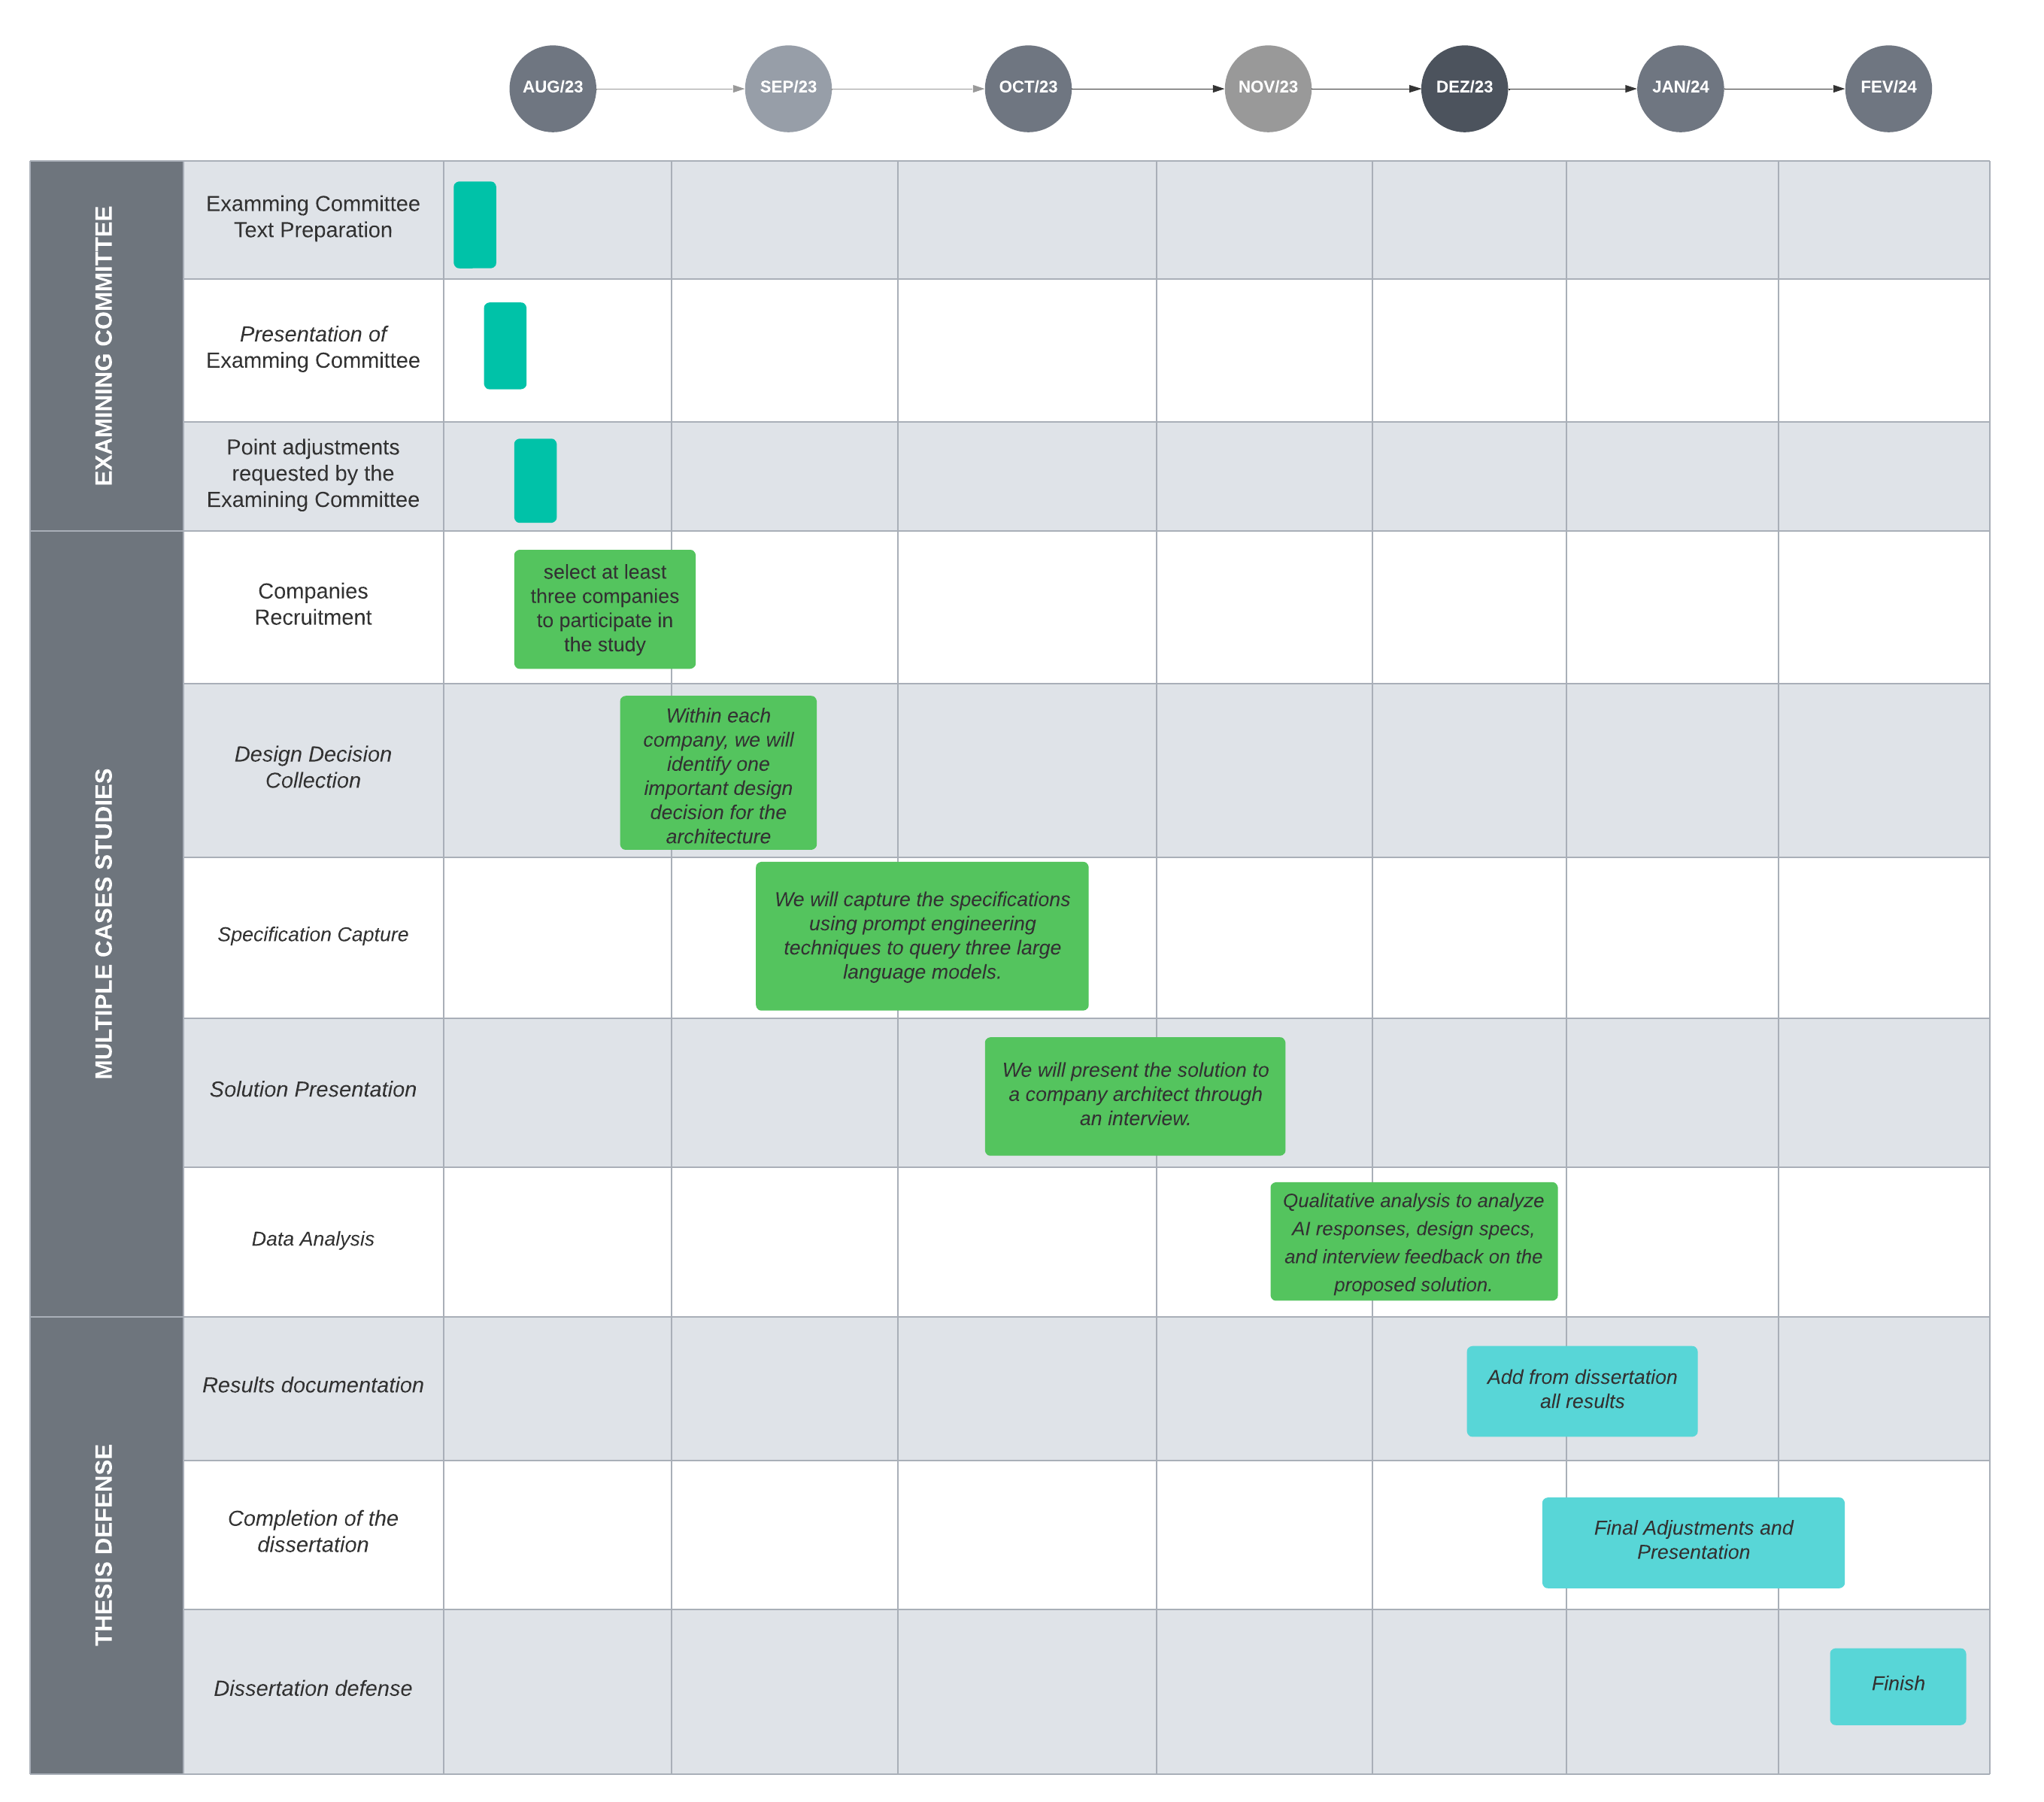
\includegraphics[width=1.0\textwidth]{figures/planning.png}
\objectsource{\objectsourceauthor}
\end{figure}
% End Figure ---------------------------

As September 2023 arrives, we enter the next phase of the project. Our main task now is to identify a significant design decision from the architecture of each participating company. This step is crucial as these decisions will form the foundation of our future analysis. In addition, this month marks the presentation to the Examining Committee, wherein they may request adjustments to the research direction or methodology.

In October, the project will enter a crucial phase of capturing specifications. With the help of prompt engineering techniques, three extensive language models are used to extract essential information. This method of gathering data provides a comprehensive and detailed understanding of the design choices made by each company.

In November, we will present our analyzed solutions to the architects from each company. We will conduct this through an interview, where we can discuss the results and their implications.

In December, the task shifted towards the deep analysis of the data gathered. A qualitative approach is employed to dissect the AI responses, design specifications, and feedback from the interview with the company architects. This stage is crucial for gaining insights and drawing valid conclusions from the data collected.

As the new year begins in January 2024, the focus shifts towards wrapping up the project. The results from the data analysis are meticulously documented and integrated into the more extensive dissertation. It is a period for final adjustments, where every detail is refined, every conclusion is evaluated, and the dissertation takes its final form.

Then, the moment of reckoning arrives in February 2024. After months of diligent work, the dissertation is ready for defense. It is presented to the examining Committee, defending the methodology, findings, and conclusions derived from the research. The defense marks the culmination of months of rigorous research and is a moment to articulate and defend the insights drawn from the data.

As with any research project, the timeline and progression of work depend on several factors. Company availability and compliance, committee feedback timing, and depth of data analysis all play significant roles. Flexibility and contingency planning will help us navigate through any unexpected delays or complications that arise.